\begin{figure}[H]
    \centering
    \begin{subfigure}{0.3\textwidth}
        \centering
        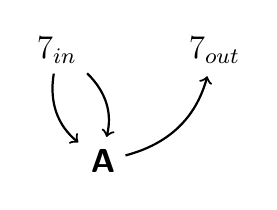
\begin{tikzpicture}[->,shorten >=1pt,auto,node distance=2cm,
                            thick,main node/.style={font=\sffamily\large\bfseries}]

        % Define vertices
        \node[main node] (7) {$7_{in}$};
        \node[main node] (77) [right of=7] {$7_{out}$};
        \node[main node] (A) [below left of=77] {A};

        % Draw edges
        \path[every node/.style={font=\sffamily\small}]
            (7) edge[bend right] (A)
            (7) edge[bend left] (A)
            (A) edge[bend right] (77);

        \end{tikzpicture}
        \caption{\textsc{STN}(R') after \textsc{Condense}}
    \end{subfigure}
    \begin{subfigure}{0.3\textwidth}
        \centering
        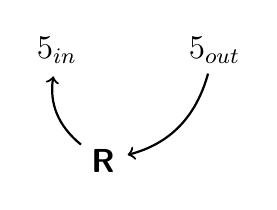
\begin{tikzpicture}[->,shorten >=1pt,auto,node distance=2cm,
                            thick,main node/.style={font=\sffamily\large\bfseries}]

        \node[main node] (5) {$5_{in}$};
        \node[main node] (55) [right of=5] {$5_{out}$};
        \node[main node] (R) [below left of=55] {R};

        \path[every node/.style={font=\sffamily\small}]
            (55) edge[bend left] (R)
            (R) edge[bend left] (5);

        \end{tikzpicture}
        \caption{\textsc{STN}(A)}
    \end{subfigure}
    \begin{subfigure}{0.3\textwidth}
        \centering
        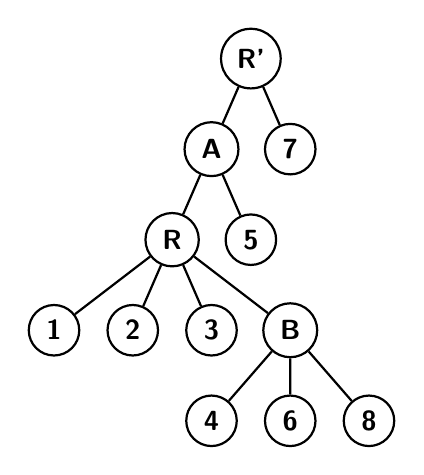
\begin{tikzpicture}[level distance=1.15cm,
                            level 1/.style={sibling distance=1cm},
                            level 2/.style={sibling distance=1cm},
                            thick,main node/.style={circle,draw,font=\sffamily\bfseries}]

        % Define vertices
        \node[main node] (R') {R'}
            child {node[main node] (A) {A}
                child {node[main node] (R) {R}
                    child {node[main node] (1) {1}}
                    child {node[main node] (2) {2}}
                    child {node[main node] (3) {3}}
                    child {node[main node] (B) {B}
                        child {node[main node] (4) {4}}
                        child {node[main node] (6) {6}}
                        child {node[main node] (8) {8}}
                    }
                }
                child {node[main node] (5) {5}}
            }
            child {node[main node] (7) {7}};
        \end{tikzpicture}

        \caption{updated SCC-tree}     
    \end{subfigure}
    \caption{\textsc{STN}(R'), \textsc{STN}(A) and updated SCC-tree}
    \label{fig:stn_a_and_updated_scc_tree}
\end{figure}
 